 
 \documentclass[manuscript,screen=true, review, anonymous]{acmart}
 
 \usepackage[utf8]{inputenc}
 \usepackage{xspace}
 \usepackage{balance}
 \usepackage{amsmath,amsfonts,mathtools,amsthm}
 \usepackage{algorithmic}
 \usepackage{algorithm}
 
 \usepackage{balance}
 \usepackage[english]{babel}
 \usepackage{blindtext}
 \usepackage{amsthm,amsmath,array,colortbl,graphicx,multirow}
 \usepackage{comment}
 \usepackage{balance}
 \usepackage{tikz}
 \usepackage{amsmath}
 \usetikzlibrary{patterns} %
 \usepackage{algorithm}
 \usepackage[font={footnotesize}]{subcaption}
 \usepackage[font={footnotesize}]{caption}
 \usepackage{breakcites}
 \usepackage{booktabs}
 \usepackage{diagbox}
 \usepackage{xcolor}
 \usepackage{colortbl}
 \usepackage{cleveref}
 \usepackage{enumitem}
 
 \mathchardef\mhyphen="2D
 
 \title{Online Balanced Graph Partitioning: Optimizations for Large Clusters}
 
 
 \author{Maciej Pacut}
 \email{maciej.pacut@univie.ac.at}
 \orcid{0000-0002-6379-1490}
 \affiliation{%
 \institution{Faculty of Computer Science, University of Vienna}
 \country{Austria}
 }
 
 
 \author{Mahmoud Parham} 
 \email{mahmoud.parham@univie.ac.at}
 \orcid{0000-0002-6211-077X}
 \affiliation{%
 \institution{Faculty of Computer Science, University of Vienna}
 \country{Austria}
 }
 
 \author{Stefan Schmid} 
 \email{stefan_schmid@univie.ac.at}
 \affiliation{%
 \institution{Faculty of Computer Science, University of Vienna}
 \country{Austria}
 }
 
 \copyrightyear{2020} 
 \acmYear{2020} 
 \setcopyright{acmlicensed}
 \acmConference{DISC '20}{October 12-16, 2020}{Freiburg, Germany}
 
 \keywords{online algorithms, competitive analysis, graph partitioning, clustering}
 \acmISBN{}\acmPrice{}
 \acmDOI{}
 
 \ccsdesc[500]{Networks~Network algorithms}
 \ccsdesc[300]{Computer systems organization~Cloud computing}
 \ccsdesc[300]{Computer systems organization~Distributed architectures}
 
 %%%%%%%%%%%%%%%%%%%%%%%%%%%%%%%%%%%%%%%%%%%%%%%%&&
 %%%%%%%%%%%%%%%%%%%%%%%%%%%%%%%%%%%%%%%%%%%%%%%%&&
 %  our macros start
 %%%%%%%%%%%%%%%%%%%%%%%%%%%%%%%%%%%%%%%%%%%%%%%%&&
 %%%%%%%%%%%%%%%%%%%%%%%%%%%%%%%%%%%%%%%%%%%%%%%%&&
 
 \newcommand{\OPT}{\textsf{OPT}\xspace}
 \newcommand{\ALG}{\textsf{ALG}\xspace}
 \newcommand{\PPL}{\textsf{PPL}\xspace}
 \newcommand{\OBRP}{BRP}
 \newcommand{\PPOBRP}{PP-BRP}
 \newcommand{\dist}{\textsf{dist}}
 \newcommand{\TAlg}{{\ensuremath{\textsf{ALG}_{3}}}\xspace}
 
 \newcommand{\comm}{\textsc{comm}}
 \newcommand{\OFF}{\textsc{Off}\xspace}
 \newcommand{\Rep}{\textsc{Rep}}
 
 
 
 
 \newtheorem{claim}{Claim}
 \newtheorem{fact}{Fact}
 \newtheorem{rem}{Remark}
 \newtheorem{observation}{Observation}
 \newtheorem{property}{Property}
 
 
 \DeclarePairedDelimiter\pair{(}{)}
 \DeclarePairedDelimiter\set{\{}{\}}
 
 \DeclarePairedDelimiter{\ceil}{\lceil}{\rceil}
 \DeclarePairedDelimiter{\floor}{\lfloor}{\rfloor}
 
 \newcommand\mahmoud[1]{\color{orange}\textbf{\\ Mahmoud: #1}\\\color{black}}
 \newcommand\stefan[1]{\color{blue}\textbf{\\ Stefan: #1}\color{black}}
 \newcommand\maciek[1]{\color{brown}\textbf{\\ Maciek: #1}\color{black}}
 %\newcommand\maciek[1]{}
 
 
 \newcommand{\todo}[1]{\noindent\color{brown}{todo: #1}\color{black}}
 
 \begin{CCSXML}
	<ccs2012>
	<concept>
	<concept_id>10003033.10003068</concept_id>
	<concept_desc>Networks~Network algorithms</concept_desc>
	<concept_significance>500</concept_significance>
	</concept>
	<concept>
	<concept_id>10010520.10010521.10010537.10003100</concept_id>
	<concept_desc>Computer systems organization~Cloud computing</concept_desc>
	<concept_significance>300</concept_significance>
	</concept>
	<concept>
	<concept_id>10010520.10010521.10010537</concept_id>
	<concept_desc>Computer systems organization~Distributed architectures</concept_desc>
	<concept_significance>300</concept_significance>
	</concept>
	</ccs2012>
\end{CCSXML}

% for my small screen
%\setlength{\textwidth}{8cm}

\begin{document}

\begin{abstract}
	Distributed   applications,  including  batch  processing, streaming, scale-out databases,
	or machine learning, generate a significant amount of network traffic. By collocating frequently communicating nodes (e.g., virtual machines) on the same clusters (e.g., server or rack), the network load can be reduced and application performance improved. 
	However, as the communication pattern is a priori unknown and may change over time, it needs to be learned efficiently, in an online manner.
	%
	This paper revisits the online 
	balanced repartitioning problem 
	(introduced by Avin et al.~at DISC 2016)
	which asks for an algorithm that strikes
	an optimal tradeoff between the benefits
	of collocation (i.e., lower network load) 
	and its costs (i.e., migrations). 
	%
	Our first contribution is a significantly improved
	lower bound of $\Omega(k\cdot \ell)$ on the
	competitive ratio, where $\ell$ is the number
	of clusters and $k$ is the cluster size,
	even for a scenario in which the communication
	pattern is static and can be perfectly partitioned;
	we also provide a tight upper bound 
	of $O(k\cdot \ell)$ for this scenario.
	In addition, we present a tight upper bound
	of $\Theta(\ell)$ for $k=3$,
	for the general model in which the
	communication pattern can change arbitrarily
	over time. 
\end{abstract}

\maketitle

\renewcommand{\shortauthors}{M.~Pacut, M.~Parham, S.~Schmid}

\section{Introduction}

\noindent \textbf{Motivation and model.}
The \emph{balanced repartitioning} problem (\OBRP{})
is a fundamental learning problem
that finds applications in the context of
distributed systems optimization~\cite{repartition-disc}. We are given a set $V$ of $n$ nodes 
(e.g., virtual machines or processes),
initially arbitrarily partitioned into $\ell$~clusters
(e.g., servers or entire racks),
each of size~$k$.
The nodes interact using
a sequence of pairwise communication requests
$\sigma = (u_1,v_1),$ $(u_2,v_2),$ $(u_3,v_3), \ldots$,
where a pair $(u_t,v_t)$ indicates that nodes $u_t$ and $v_t$ exchange a~certain amount of data.
Nodes in $C \subset V$ are \emph{collocated}
if they reside in the same cluster.

An algorithm serves a communication request between two nodes
either \emph{locally} at cost~0
if they are collocated,
or \emph{remotely} at cost~1
if they are located in different clusters.
We refer to these two types of requests as \emph{internal}
and \emph{external} requests, respectively.
Before serving a request,
an online algorithm may perform a \emph{repartition},
%(i.e., \emph{reconfigure}).
i.e.,
it may move (``migrate'') some nodes into clusters different from their current clusters, while respecting the capacity of every cluster. 
Afterwards, 
the algorithm serves the  request.
The cost of migrating a node from one cluster to another
is~$\alpha \in \mathbb{Z}^+$.
\maciek{Why restrict $\alpha$? It should just be positive}
For any algorithm $\ALG$,
its cost,
denoted by $\ALG(\sigma)$,
is the total cost of communications and
the cost of migrations performed by $\ALG$ while serving the sequence $\sigma$.

In addition to the general model, we study a simplified Perfect Partition model (also studied by Henzinger et al.~\cite{sigmetrics19_partitioning} (SIGMETRICS 2019)) that we consider for a stronger lower bound.
There, we assume that $\sigma$
reveals the edges of a static graph
that can be perfectly partitioned
(no external requests are required). 

The general model, where $\sigma$ can be arbitrary
was the original problem introduced
by Avin et al.~\cite{repartition-disc} at DISC 2016.
For simplicity, we will refer to the Perfect Partition
model as the \emph{learning} model (as
one has to learn the static communication graph) 
and to the original as the \emph{repartitioning} model (as one continuously adjusts the partition in response to changing communication graph).


\noindent \textbf{Contributions.}
We provide an improved lower bound 
of $\Omega(k\cdot\ell)$ on the competitive ratio of any online deterministic online algorithm 
even in the learning model;
the best known lower bound so far was $\Omega(k)$,
even for a more general model~\cite{repartition-disc}.
We also present an asymptotically optimal, 
$O(k\cdot \ell)$-competitive algorithm
for the learning model.
For the repartitioning model, we present  
an asymptotically optimal,
$\Theta(\ell)$ algorithm for $k=3$;
the best known upper bound 
so far was $O(\ell^2)$~\cite{repartition-disc}.
Then, we present a strictly $6$-competitive algorithm for $k=2$.
In addition, we show a new, improved analysis of the algorithm from \cite{repartition-disc} that depends on the solutions to an interesting combinatorial problem (see Section~\ref{ssec:cascade}, The Cascade Problem).
%
The overview of known results is in Table~\ref{tab:overview}.

\begin{table*}
	\centering
	\renewcommand{\arraystretch}{1.5}
	\begin{tabular}{>{\centering\arraybackslash}p{4.5cm}|>{\centering\arraybackslash}p{4.5cm}>{\centering\arraybackslash}p{4.5cm}}
		\rowcolor{gray!50}
		\textbf{Variant} & \textbf{ Lower bound} &\textbf{Upper bound}\\ \hline 
		\textbf{$k=2$}& 3\hspace{0.3cm}\cite{repartition-disc} & 6\hspace{0.3cm}(\S \ref{sec:k2}) \\ 
		\rowcolor{gray!25}
		\textbf{$k=3$}&  $\ell - 3/2$ \hspace{0.3cm}(\S \ref{sec:lowerbound})& $54\cdot \ell $\hspace{0.3cm}(\S \ref{sec:k3})\\
		$k > 3$ & $(k\cdot \ell - k - \ell) / 2$\hspace{0.3cm}(\S  \ref{sec:lowerbound})&$O(k \cdot \ell \cdot \min \{ k \cdot \ell, \Rep(k, \ell) \})$\hspace{0.3cm} (\S \ref{sec:k3}) \\
		\rowcolor{gray!25}
		Perfect partition & $(k\cdot \ell - k - \ell) / 2$\hspace{0.3cm}(\S  \ref{sec:lowerbound})&$2(k -1 )\cdot \ell$\hspace{0.3cm} (\S \ref{sec:ppl}) \\
	\end{tabular}
	\caption{Overview of known results and the results provided in this paper. By $\Rep$ we denote the cost of a single component repartition, and we elaborate on this in Section~\ref{sec:k3}
	}
	\label{tab:overview}
	\vspace{-7mm}
\end{table*}

\noindent \textbf{Related work.}
The existing results in~\cite{repartition-disc}
and~\cite{sigmetrics19_partitioning}
primarily focus on a model where 
the online algorithm can use augmentation,
i.e., has slightly larger clusters than the offline 
algorithm. In contrast, in our paper, we focus
on a scenario where the nodes need to be
perfectly balanced among the clusters.
The problem has also been studied in a weaker
model where the adversary can only sample
requests from a fixed distribution~\cite{stochastic-ring}.
For clusters of size $2$ (i.e., $k=2$), 
it is known that a $7$-competitive algorithm exists~\cite{repartition-disc} with large ($\Omega(\ell^2)$) additive constant.

%More generally, the model is related to online
%caching~\cite{SleTar85,FKLMSY91,McGSle91,AcChNo00},
%see~\cite{repartition-disc} for a discussion.
%The static offline version of~the~problem, called the
%\emph{$\ell$-balanced graph partitioning problem} is 
%NP-complete, and cannot even be approximated within %any finite factor unless P
%= NP~\cite{AndRae06}. 

\section{Preliminaries.}

Across this paper, we often refer to groups of communicating nodes.
As this concept is used differently in the lower bound and the upper bounds, we name them differently to avoid confusion.

\noindent
\textbf{Components.}
In our algorithms, a~\emph{component} is a subset of frequently communicating nodes.
We maintain all nodes of each component collocated in one cluster~\cite{repartition-disc}.
If we need to move a node, we move the whole component that contains it.
We maintain a balanced partition of our components, a similar concept to partition of integers into sets with equal sum (\maciek{TODO: cite}).
In contrast, our partition is time-varying: communicating components are merged into one, and we adjust the partition.

\noindent
\textbf{Ground sets.}
In the lower bound, a~\emph{ground set} is a group of nodes that start communicating if an algorithm splits them (places at different clusters).
Their role is to ensure that the algorithm maintains a partition of ground sets.
We emphasize that ground sets are revealed only upon their nodes are split.
\maciek{Other names: division, segmentation, alignment, formation}

%We say that the request $(u,v)$ is \emph{external}, if the algorithm is in the configuration, where $u$ and $v$ are located at different clusters.
%This is achieved by opting a sequence of  partitions (a.k.a.~configurations)
%such that frequently communicating nodes (from different clusters)
%are relocated to the same cluster before they inflict too much communication cost.
%A \emph{reconfiguration} (i.e.,\emph{ re-partitioning})
%is performed by migrating nodes between clusters,
%at the total cost of individual node migrations.
%The objective is to jointly minimize communication and migration costs while serving the sequence.

We say that a component or a ground set is \emph{trivial}, if it contains exactly one node.
We say that the node that belongs to trivial component or a ground set is \emph{alone}.
We say that a~configuration is \emph{component respecting}
if the nodes belonging to the same component are collocated.
Similarly, we define a \emph{ground-set-respecting} configuration.

\maciek{Eviction - introduce.}


\section{The Learning Problem} %$\Omega(k\cdot \ell)$ for Competitive Ratio of Any Deterministic Algorithm}

\maciek{TODO: Intro to the learning problem is missing. What is the problem definition. How is it different from the general problem. Emphasize the fact that OPT is constrained not to migrate.}

At the end of this section, we discuss an asymptotically optimal upper bound.


\subsection{Lower bound.}

\label{sec:lowerbound}


In this section, we provide a lower bound $\Omega(k\cdot \ell)$ for the competitive ratio of any deterministic online algorithm.
It is oblivious to the choice of the reconfiguration cost $\alpha$, and we compare the number of performed node exchanges.
The lower bound requires $k\geq 3$.
Note that for $k=2$, a lower bound of $3$ is known \cite{repartition-disc}.




\begin{figure}[H]
	\centering
	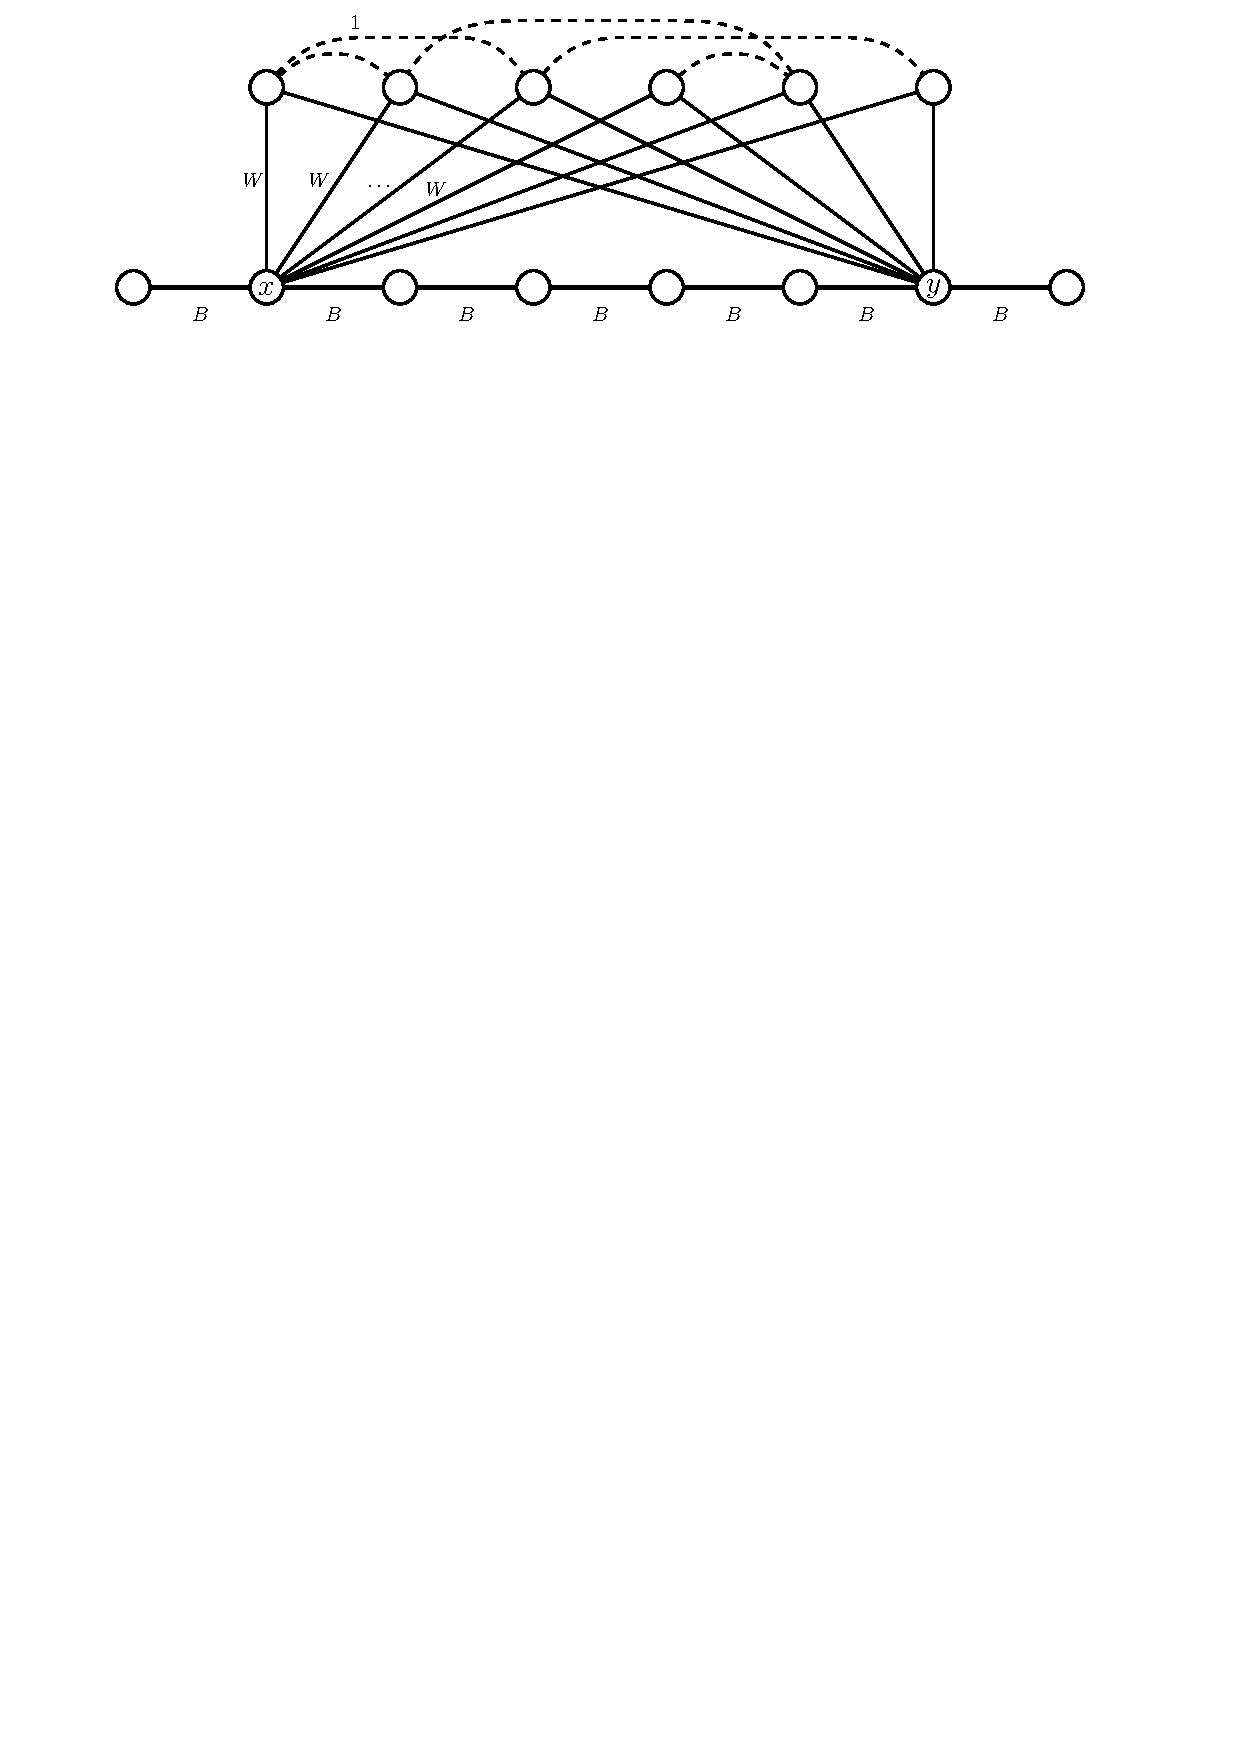
\includegraphics[width=0.3\textwidth]{figs/substitute}
	\caption{Example figure of the construction of the LB and growing components.}
	\label{fig:nptree-construction}
\end{figure}


The adversary constructs ground sets in reaction to choices of a deterministic online algorithm.
The algorithm does not know the ground set before they are revealed, and it may split some of them while evicting nodes.

Once we construct a ground set, it lasts until the end of the input sequence.
If the algorithm splits any pair of nodes of a ground set, the adversary issue requests to any pair of split nodes.

We construct the ground sets in a way that they always form a balanced partition of nodes.
This way, the optimal algorithm moves to a~ground-set-respecting configuration, and serves all requests for free.
(This implies that the algorithm must eventually move to any ground-set-respecting configuration if it is competitive.)

First, we construct a ground set of size $k-1$ on one of the clusters.
In any configuration, there exists a node that accompanies it.
We only issue requests between such accompanying (time-varying) node, and any node that was initially collocated with it.
Repeating such requests, almost every node must visit this cluster.
In comparison, \OPT performs one migration.

\begin{theorem}
	\label{th:lowerbound}
	The competitive ratio of any deterministic online algorithm for \OBRP{} is  $(k \cdot \ell - k - \ell) / 2 = \Omega(k\cdot \ell)$ for any $k\geq 3$ and for any $\ell \geq 2$.
\end{theorem}

\begin{proof}
	Fix any online algorithm \ALG{}.
	Let $I(C)$ denote the cluster where nodes of ground set $C$ are located initially.
	\maciek{A problem with the definition! The first pair does not have the same initial location of its nodes.}
	Initially all nodes are single (they belong to their own trivial ground sets).

	We distinguish a cluster $S_1$, where we form a ground set of size $k-1$.
	We never dismiss any constructed ground set.
	Each cluster host exactly $k$ nodes, hence in any configuration of \ALG, there exists a single alone node in $S_1$.

	We construct a ground set containing this alone node (and some other node).
	Precisely, let $x_0$  be the alone node from $S_1$ and let $y_0$ be an arbitrary node that does not reside in $S_1$.
	First,
	we construct a ground set $\{x_0, y_0\}$.
	Since \ALG{} has them split, the adversary produces an external request.
	Since $S_1$ contains a ground set of size $k$, \ALG{} must collocate $\{x_0, y_0\}$ in another cluster.
	To preserve a feasible partition of nodes into clusters,
	\ALG must replace $x_0$ with another single node $x_1$.
	
	We continue to construct ground sets containing the current alone node from $S_1$.
	Precisely, we merge the ground sets of $x_1$ and the largest ground set $C$ s.t.~$I(C) = I(x_1)$.
	To preserve a feasible partition of nodes into clusters,
	\ALG{} must collocate $x_1$ and $C$ in a~cluster other than $S_1$ and
	consequently replace $x_1$ with another alone node $x_2$.

	We end this procedure prematurely (before all nodes visit $S_1$) to keep \OPT's cost low.
	We repeat merging the component of single node $x_i$ on $S_1$ and the largest component $C'$ s.t.~$I(C')=I(x_i)$,
	until there are only two single nodes left that  originate from the same cluster.
	Formally, we denote these two single nodes by $x^*, y^*$, and we have $I(x^*) = I(y^*)$, and~for any other pair of single nodes
	$x'$ and $y'$,
	we have $I(x') \neq I(y')$.
	Note that at this point there are at most $\ell+1$ single nodes left,
	otherwise, there would be more pairs of single nodes that were initially in the same cluster.
	
	Finally, we bound the cost of \OPT.
	Given this sequence of requests,
	\OPT migrates $\set{x_0,y_0}$ to the cluster $I(x^*)$ by
	swapping $\set{x_0,y_0}$ with $\set{x^*,y^*}$.
	Hence,
	OPT pays for $2$ node swaps and
	\ALG{} incurs at least one swap for each node in the sequence $X := x_0, x_1,\dots$.
	We exclude at most $(k-1) + ( \ell+1)$ nodes out of $k \cdot \ell$ nodes,
	therefore $|X| \geq k \cdot \ell - k - \ell$ \maciek{elaborate on exclusion?}.
	Finally, $\ALG/\OPT \geq (k \cdot \ell - k - \ell) / 2\in \Omega(k\cdot\ell)$.
\end{proof}

\noindent
\textbf{Remark on resource augmentation.}
The majority of work on Online Balanced Partioning so far (todo: cite) focuses on the scenerio with resource augmentation.
We note that this lower bound provides insights into this scenario as well.
Consider an instance with $k$ divisible by $3$, and construct $3$ ground sets of size $k/3$ in each cluster.
Then, apply the construction from the lower bound for $k=3$, now treating these ground sets in the way we used individual nodes.
For the resource augmentation as large as $1+1/3-\epsilon$, no more than $3$ such ground sets fit in one cluster.
Therefore, the lower bound $\Omega(\ell)$ holds.

\subsection{Upper bound.}
\label{sec:ppl}
Now we give an algorithm for a restricted variant of  \OBRP{}, named \PPOBRP{},
%\maciek{This is not sufficient! We also disallow serving requests remotely.}
where an optimal offline algorithm ($\OPT$) moves to a perfect partition
at the beginning and stays there perpetually.
\maciek{Already mention that the LB is for that scenario}
%We refer this variant as \PPOBRP{}.
The task of an online algorithm for \PPOBRP{} is to recover (or learn) the perfect partition while not paying too much relative to \OPT.
%
%\maciek{This is not a valid description of the model. We need the assumption that collocation is needed in our model. Otherwise OPT would just serve some requests remotely, and our analysis would not hold.}
The first request between any two non-collocated nodes reveals an edge of the communication graph.
Our online algorithm collocates them immediately and never separates them since by assumption \OPT does the same.
Revealed edges, up to any point in the sequence,
induce some connected subgraphs which grow as components \maciek{rewrite sentence, expand}.
%An algorithm that always  keeps nodes belonging to the same component collocated is \emph{component respecting}.

\maciek{The remainder of the paper used "configuration C" to denote the partition P. Easiest to adjust here.}

We assume \OPT begins with the initial configuration
$P_I = I_1, \dots, I_{\ell}$ and moves to the final partitioning
$P_F = F_1, \dots, F_{\ell}$.
The \emph{distance} of a configuration $P = C_1, \dots, C_{\ell}$ from the initial configuration \maciek{, denoted $\dist(P)$} is the number of nodes in $P$ that do not reside in their initial cluster.
\maciek{We might denote distance $\Delta(P)$, and the current $\Delta$ might be R (like radius).}
That is,
$\dist(P, P_I) := \sum_{j=1}^{\ell} | C_j \setminus I_j |$. 
In other words,
at least $\dist(P, P_I)/2$ node swaps are required in order to reach the configuration $P$ from $P_I$, and thus
$\OPT \geq \Delta:= \dist(P_F, P_I) $.
With each repartitioning,
\PPL moves to a configuration that minimizes the distance to the initial configuration $P_I$.
As a result,
\PPL never ends up in a configuration that is more than $\Delta$ (single-node) migrations away from $P_I$.
This invariant ensures that \PPL does not pay too much while recovering $P_F$.
%      \maciek{``re-partition'' procedure name should indicate the fact that this is a specific repartition that is close to initial partition}
We note that the $\mathit{repartition}$ at Line \ref{line:rebalance} replaces the current configuration $P$ with a~perfect partition closest to $P_I$.
Hence it never moves to a configuration beyond distance $\Delta$.
The scheme of the algorithm can be found in the Algorithm \ref{alg:PPL}.

\section{PPL Algorithm} \label{alg:PPL}
\begin{algorithm}
	\renewcommand{\algorithmicrequire}{\textbf{Input:}}
	\renewcommand{\algorithmicensure}{\textbf{Output:}}
	\begin{algorithmic}
		%        \Require 
		%        $k, \ell$,
		%        initial configuration $P_I$,
		%        sequence of  requests $\sigma_1, \dots, \sigma_N$ 
		%        \Ensure A final configuration $P_F$ 
		\STATE {For each node $v$ create a singleton component $C_v$ and add it to $\mathcal{C}$}
		\STATE{$P_0 := P_I$}
		\label{line:initcomponents}
		\FOR {each  request $\sigma_t=\{u,v\}, 1 \leq t \leq N$}
		\STATE Let $C_1 \ni u$ and $C_2 \ni v$ be the container components
		\IF{$C_1 \neq C_2$}
		\STATE {Unite the two components into a single component $C'$ and
		$\mathcal{C} = (\mathcal{C}\setminus\set{C_1, C_2}) \cup ~\set{C'}$} \label{line:mergecomponents}
		\IF{$\mathit{cluster}(C_1, P_{t-1}) \neq \mathit{cluster}(C_2, P_{t-1})$
		\COMMENT{i.e.~if not in the same cluster}    
		}       
		\STATE {$P_{t} = \mathit{repartition}(P_{t-1}, P_I, \mathcal{C})$} 
		\COMMENT{move to $P$ closest to $P_I$}
		\label{line:rebalance} 
		\ENDIF
		\ENDIF
		\ENDFOR
	\end{algorithmic}
	\caption{Perfect Partition Learner (\PPL)}
	\label{alg:ppl}
\end{algorithm}

\begin{property} \label{prop:dist<OPT}
	Let $P$ be any configuration chosen by \PPL at Line $\ref{line:rebalance}$.
	Then, $\dist(P,P_I) \leq \Delta$.
\end{property}
\maciek{The property is explained in the previous paragraph. Here, reader thinks that this is obvious and wonders why. Move closer to the exlaination text.}

\begin{lemma}	\label{lemma:rebalancecost}
	The cost of repartitioning at Line \ref{line:rebalance} is at most $2\cdot\OPT$.
\end{lemma}
\begin{proof}
	Consider the repartitioning that transforms $P_{t-1}$ to $P_t$ upon the request $\sigma_t$.
	Let $M \subset V$ denote the set of nodes that migrate during this process.
	Let $M^-$ and $M^+$ denote the subset of nodes that (respectively)
	enter or leave their original cluster during the repartitioning.    
	Then,
	$M = M^+ \cup M^-$.
	Since \maciek{at least?} $|M^-|$ nodes are not in their original cluster before the repartitioning (i.e., in $P_{t-1}$),
	the distance before the repartitioning is $\dist(P_{t-1},P_I) \geq | M^-|$.
	Analogously,
	the distance afterwards is $\dist(P_{t},P_I) \geq | M^+|$.
	Thus,
	$|M| \leq \dist(P_{t-1},P_I) + \dist(P_{t},P_I)$.
	By Property \ref{prop:dist<OPT},
	$\dist(P_{t-1},P_I) , \dist(P_{t},P_I) \leq \Delta \leq \OPT$
	and thereby we have	
	$|M| \leq 2\cdot\OPT$.
	\maciek{the comma between $\dist$ is confusing. BOTH are bounded? If so, expand the sentence and write both individual bounds.}
\end{proof}

\begin{theorem}	\label{thm:upperbound}
	\PPL reaches the final configuration $P_F$ and it is $(2\cdot k\cdot\ell)$-competitive.
	\maciek{Do not hide that we have $2(k-1)\ell$ in the theorem. This is a better bound.}
\end{theorem}
\begin{proof}
	On each inter-cluster request,
	the algorithm enumerates all $\ell$-way partitions of components
	that are in the same (closest) distance of $P_I$.
	That is, 
	once it reaches a configuration $P$ at distance $\Delta = \dist(P, P_I)$,
	it does not move to a configuration
	$P', \dist(P', P_I) > \Delta$,
	before it enumerates all configurations at distance $\Delta$.
	Therefore,
	\PPL eventually reaches $\Delta=\OPT$ and the configuration $P_F$.
	%    including the request that completes revealing of all components that are collocated in $P_F$.
	There are at most $(k-1)\cdot\ell < k\cdot\ell $ calls   to $\mathit{repartition}$
	(i.e., the number of internal edges in $P_F$).
	\maciek{Clarify why the number of internal edges bound the number of repartitions.}
	By Lemma \ref{lemma:rebalancecost},
	each repartition costs at most $2\cdot\OPT$.
	The total cost is therefore at most $2\cdot\OPT\cdot k\cdot\ell$, which implies the competitive ratio.
	%    \mahmoud{This is the cost of moving and the cost of remote comm. is not counted.
	%    	So it is 4-competitive (?)}
\end{proof}

% In Section~\ref{sec:lowerbound} we constructed a $\Omega(k \cdot \ell)$ for \OBRP{}.
% Note that the lower bound holds also in the perfect partition model, as the constructed input sequence allows \OPT to move to a perfect partition.
% The corollary is that PPL is optimal.

\section{The Online Problem}
\label{sec:k3}


\maciek{Not precise name? Both the learning problem and the general one is online.}

\maciek{Start with referencing the table of results, saying that some results are known already in the literature. And emphasize here that we now have an improved lower bound from the previous section, as that model was a subproblem.}

Let us now discuss the general online
model where the request sequence
can be arbitrary. We show that the classic \emph{rent-or-buy} approach~\cite{karlin-ski-rental} allows obtaining an optimal algorithm for $k=3$.
Upon receiving $\alpha$ requests between a pair of nodes, we collocate them in one cluster until the end of a phase (that we define precisely later).

\maciek{Rewrite above paragraph to say that our algorithm is essentially DET from DISC16, with concretised reconfiguration strategy (i.e., an arbitrary one among the minimum cost reconfigurations)}

\maciek{Better name than DET? Currently it is \TAlg, hence it is wrong}

\subsection{Improved analysis of the component-based algorithm}


%We define the algorithm \TAlg in the following way.
Now we describe the algorithm \TAlg.
It partitions nodes into components, and
initially, each node belongs to its own singleton component.
For each pair of nodes, \TAlg maintains a counter, initiated to $0$. 
Upon receiving a request to a pair that is not collocated in one cluster, it increases their counter by $1$.
If the counter for a pair $(u,v)$ reaches $\alpha$, \TAlg merges the components of $u$ and $v$, and moves to the closest component respecting partitioning.
If no such partitioning exists, \TAlg resets all components to singletons, resets all counters to $0$, and ends the phase.

\maciek{Emphasize the difference to DET: "Modification is the following: when repartition is necessary, move to \emph{the closest} perfect partition of components."}




\begin{figure}[H]
	\centering
	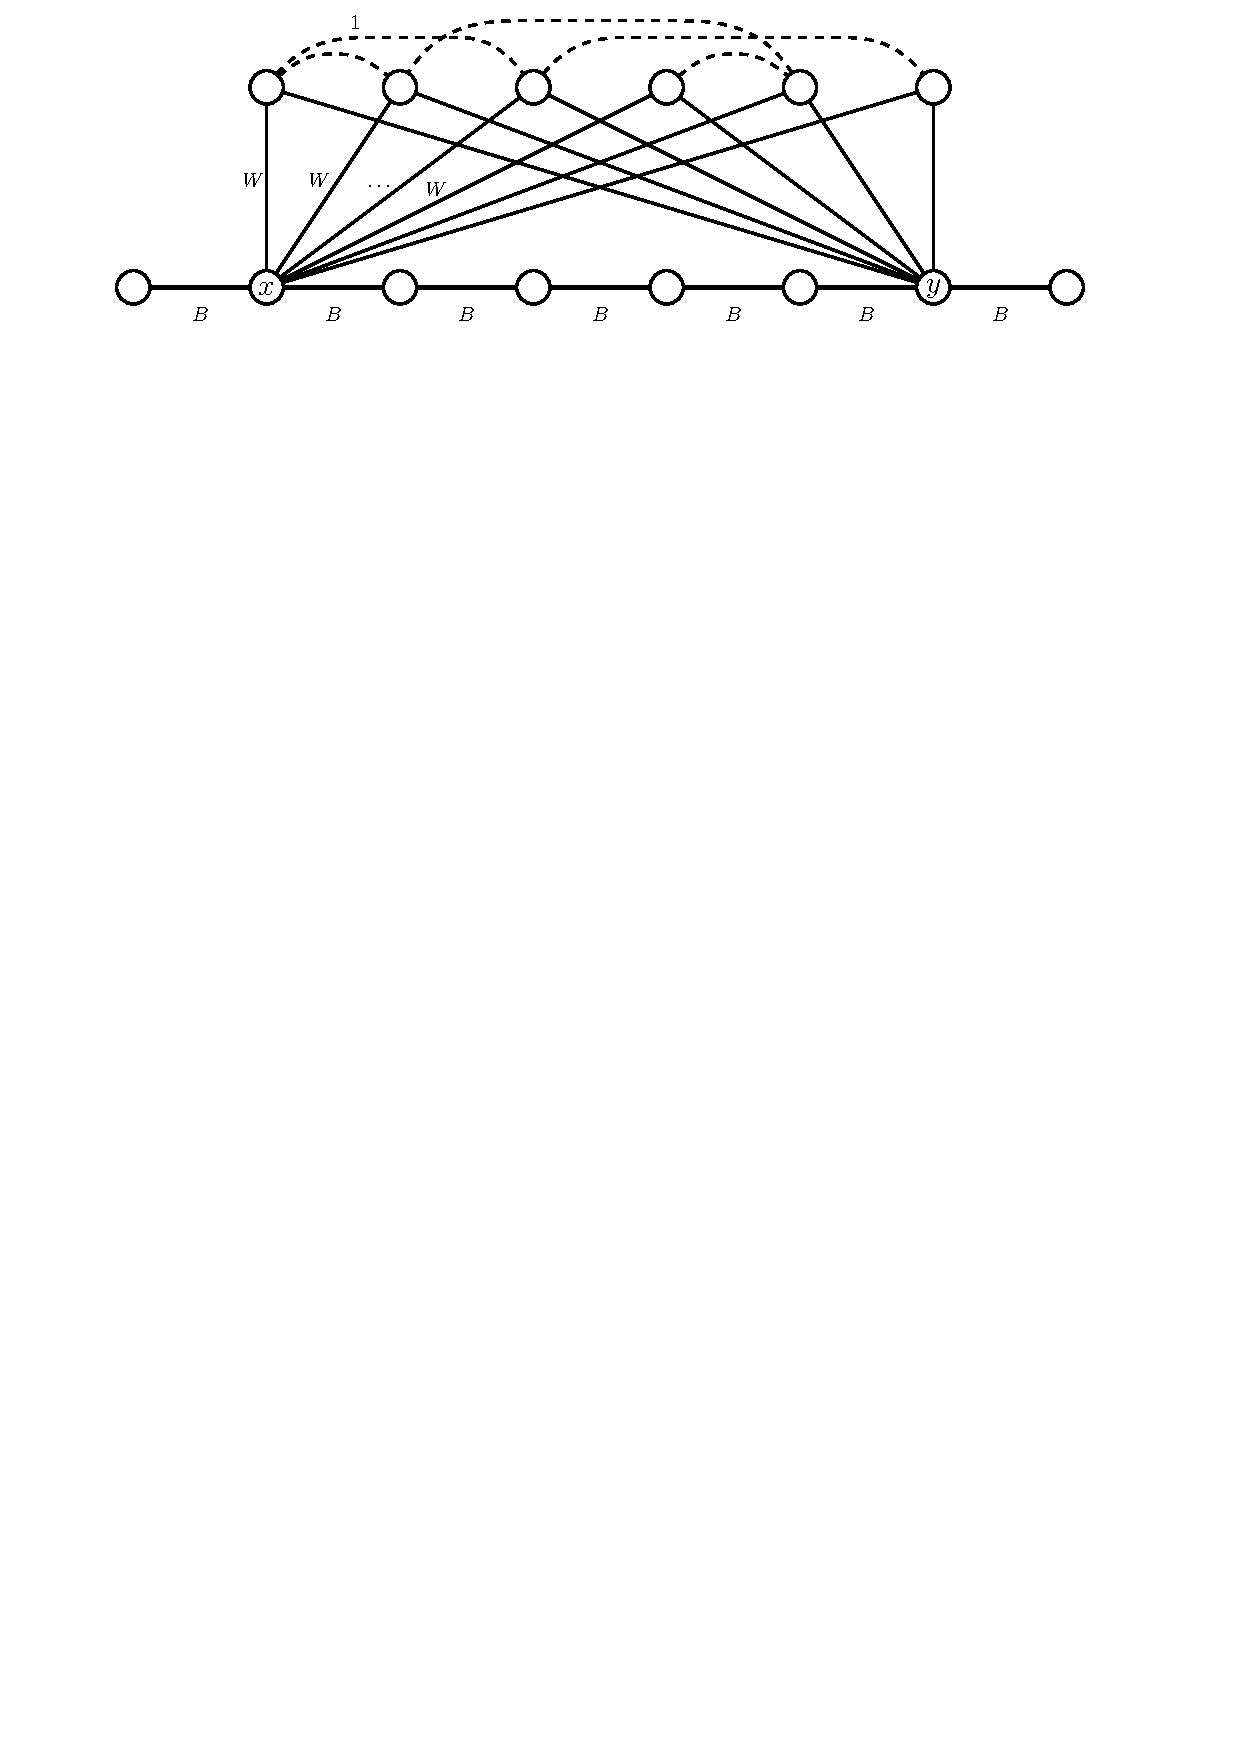
\includegraphics[width=0.3\textwidth]{figs/substitute}
	\caption{an unsaturated edge that is inside a component}
\end{figure}



\begin{theorem}
	\TAlg is $O(\ell)$-competitive.
	\maciek{Proposed new formulation (current version is all about k=3 still): Let Reconf(k,l) be a bound on the cost of a single reconfiguration. Then \TAlg is $O(Reconf(k,l)\cdot k \cdot \ell)$-competitive.}
\end{theorem}
\begin{proof}
	Fix a completed phase, and consider the state of \TAlg's counters at the end of it.
	We consider the incomplete phase later in this proof.
	
	As \TAlg is component respecting, it never increases any counter above $\alpha$.
	We say that the pair $(u, v)$ is \emph{saturated} if the counter has value $\alpha$, and \emph{unsaturated} otherwise \maciek{Rename: saturated/unsaturated edge instead of a pair}.
	Let $\sigma$ be the input sequence that arrived during the phase.
	Let $\sigma_{cost}$ be the requests that at the moment of arrival were external requests for \TAlg (these are the only requests that incurred a cost for \TAlg).
	In our analysis, we partition $\sigma_{cost}$ into subsequences $\sigma_I$ and $\sigma_E$.
	The sequence $\sigma_I$ (inter-component requests) are the requests from $\sigma_{cost}$ issued to pairs that belong to the same component of \TAlg at the end of the phase.
	The sequence $\sigma_E$ (extra-component requests) denotes the requests from $\sigma_{cost}$ that do not appear in $\sigma_I$.
	
	
	%Let $A^I$ be the cost of (extra-cluster) communication incurred in this phase by \TAlg between pairs that belonged to the single component at the end of the phase.
	%Let $A^E$ be the cost of (extra-cluster) communication incurred in this phase between the nodes that belong to different components at the end of this phase.
	Let $\TAlg(M)$ be the cost of migrations performed by \TAlg in this phase.
	\TAlg performs at most $2 \ell$ component merge operations, as
	exceeding this number means that a component of size $4$ exists, and the phase should have ended already.
	Combining this with Lemma~\ref{lem:1req} gives us $\TAlg(M) \leq 8\alpha\cdot\ell$ (recall that an exchange costs $2\alpha$).
	%Together with Lemma~\ref{lem:1req}, this allows us to bound the cost of migrations, $\TAlg(M) \leq 6\cdot\alpha\cdot\ell$.
	
	Now we bound $\TAlg(\sigma_I)$.
	A~cluster of type $C_3$ contributes at most $3 \alpha - 1$ to $\TAlg(\sigma_I)$, as $2$ of pairs of nodes from the component are saturated and contribute $\alpha$ each, and the third, unsaturated pair contributes at most $\alpha-1$.
	Other cluster types contribute less: $C_1$ contributes $0$ and $C_2$ contributes $\alpha$.
	Summing this over all $\ell$ clusters gives us $\TAlg(\sigma_I) \leq (3 \alpha-1)\cdot \ell \leq 3\alpha\cdot\ell$.
	
	%We bound $A^E$ by $k^2 \cdot (\alpha - 1)$, as no more than $k^2$ pairs are unsaturated, and each of them contributes at most $\alpha -1$.
	%\maciek{not needed most likely}
	
	Moreover, \TAlg paid for all requests from $\sigma_E$, and thus $\TAlg(\sigma_E) = |\sigma_E|$.
	In total, the cost of \TAlg is at most $\TAlg(\sigma_I) + \TAlg(\sigma_E) + \TAlg(M) \leq 11\alpha\cdot \ell + |\sigma_E|$ during this phase.
	
	\medskip
	
	Now we lower-bound the cost of $\OPT$.
	By $\OPT(\sigma_I)$ and $\OPT(\sigma_E)$ we denote the cost of $\OPT$ on these input sequences (defined with respect to components of \TAlg in this phase).
	By $\OPT(M)$ we denote the cost of migrations performed by $\OPT$ in this phase.
	
	We split the cost of $\OPT$ into parts coming from serving $\sigma_I$ and $\sigma_E$.
	While serving these requests, $\OPT$ may perform migrations, and we account for them in both parts: we separately bound $\OPT$ by $\OPT(\sigma_I) + \OPT(M)$ and $\OPT(\sigma_E) + \OPT(M)$.
	Combining those bounds gives us $\OPT \geq \max\{\OPT(\sigma_I) + \OPT(M), \OPT(\sigma_E) + \OPT(M)\} \geq (\OPT(\sigma_I) + \OPT(M)) / 2 + (\OPT(\sigma_E) + \OPT(M)) / 2$.
	
	%Let $O^M$ be the cost of migrations performed by $\OPT$ during the phase.
	%Let $O^I$ be the cost of serving requests between nodes that were put in one component by \TAlg during this phase.
	%Let $O^E$ be the cost serving requests between nodes that \TAlg did not put in the same component during that phase.
	
	%First, we estimate the cost related to $\sigma_I$.
	We have $\OPT(M) + \OPT(\sigma_I) \geq \alpha$, as the phase ended when the components of \TAlg{} could not be partitioned without splitting them.
	Hence, for every possible configuration of $\OPT$, there exists a non-collocated pair of nodes with at least $\alpha$ requests between them, and
	$\OPT$ either served them remotely or performed a~migration.
	
	\medskip
	Before we bound the competitive ratio, we relate the costs of $\TAlg$ and $\OPT$ with respect to requests $\sigma_E$.
	In a~fixed configuration of $\OPT$, it may mitigate paying for requests between at most $3\ell$ pairs of nodes by collocating them in its clusters.
	Recall that $\sigma_E$ consists of requests to unsaturated pairs, and it accounts only for requests that increased the counter (i.e., external requests), thus $\OPT$ may mitigate at most $3\ell\cdot(\alpha - 1)$ requests from $\sigma_E$.
	Faced with $W := |\sigma_E| - 3\ell\cdot(\alpha-1)$ requests $\sigma_E$ that it could not mitigate, $\OPT$ served some of them remotely and possibly performed some migrations to decrease its cost.
	
	
	Now we estimate the cost of $\OPT(\sigma_E)$ while accounting savings from migrations.
	By performing a swap of nodes $(u,v)$, $\OPT$ collocates $u$ with two nodes $u', u''$, and $v$ with two nodes $v'$, $v''$.
	This may allow serving requests between $(u,u')$, $(u,u'')$, $(v,v')$ and $(v,v'')$ for free afterwards.
	As $\sigma_E$ consists of requests to unsaturated pairs, and it accounts only for external requests, there are at most $\alpha-1$ requests between each of these pairs.
	By performing a single swap that costs $2\alpha$, $\OPT$ may avoid paying the remote serving costs for at most $4 (\alpha - 1)$ requests from $\sigma_E$
	\maciek{This changes in the general case, and introduces the factor $~1/k$ in opt's cost, increasing the competitive ratio by $O(k)$}.
	Thus, for serving $\sigma_E$, $\OPT$ pays at least $\OPT(\sigma_E) + \OPT(M) \geq W \cdot \frac{2\alpha}{4 (\alpha-1)}\geq |\sigma_E| / 2 - 2 \alpha \cdot \ell$.
	From that, we obtain $|\sigma_E| \geq 2(\OPT(\sigma_E)+\OPT(M)) + 4\alpha \cdot \ell$.
	Let $E := \OPT(\sigma_E) + \OPT(M)$. Finally, we are ready to bound the competitive ratio
	\begin{equation*}
		\frac{\TAlg(\sigma)}{\OPT(\sigma)} \leq \frac{11\alpha \cdot \ell + |\sigma_E|}{\alpha/2 + E/2} \leq \frac{27\alpha\cdot\ell + 2\cdot E}{\alpha + E} \leq 27 \ell = O(\ell).
	\end{equation*}
	
	\medskip
	
	It remains to consider the last, unfinished phase.
	Consider the case, where the unfinished phase is also the first one.
	Then, we cannot charge $\OPT$ due to the inability to partition the components.
	Instead, we use the fact that \TAlg and $\OPT$ started with the same initial configuration.
	We charge $\OPT$ $\alpha$ for the first external $\alpha$ requests or a migration,
	and we follow the analysis regarding the unsaturated requests.
	If the input finished before the first $\alpha$ external requests, then \TAlg is optimal.
	\maciek{Missing second case: then we just charge opt alpha for this one edge and this is sufficient, as the cost of alg only decreases from the full phase}
	Now, consider the case, where there are at least two phases, then we split the cost $\alpha$ charged in the penultimate phase into last two phases, and follow the analysis regarding the unsaturated requests.
	This way, the competitive ratio increases at most twofold.
\end{proof}


\section{Bounding the cost of a single reconfiguration of components}

\maciek{Overview of the section, intro. Defer introducing the graph notation, the warm-up does not need it}

\subsection{Warm-up: bounding the reconfiguration for $k=3$}


\begin{figure}[H]
	\centering
	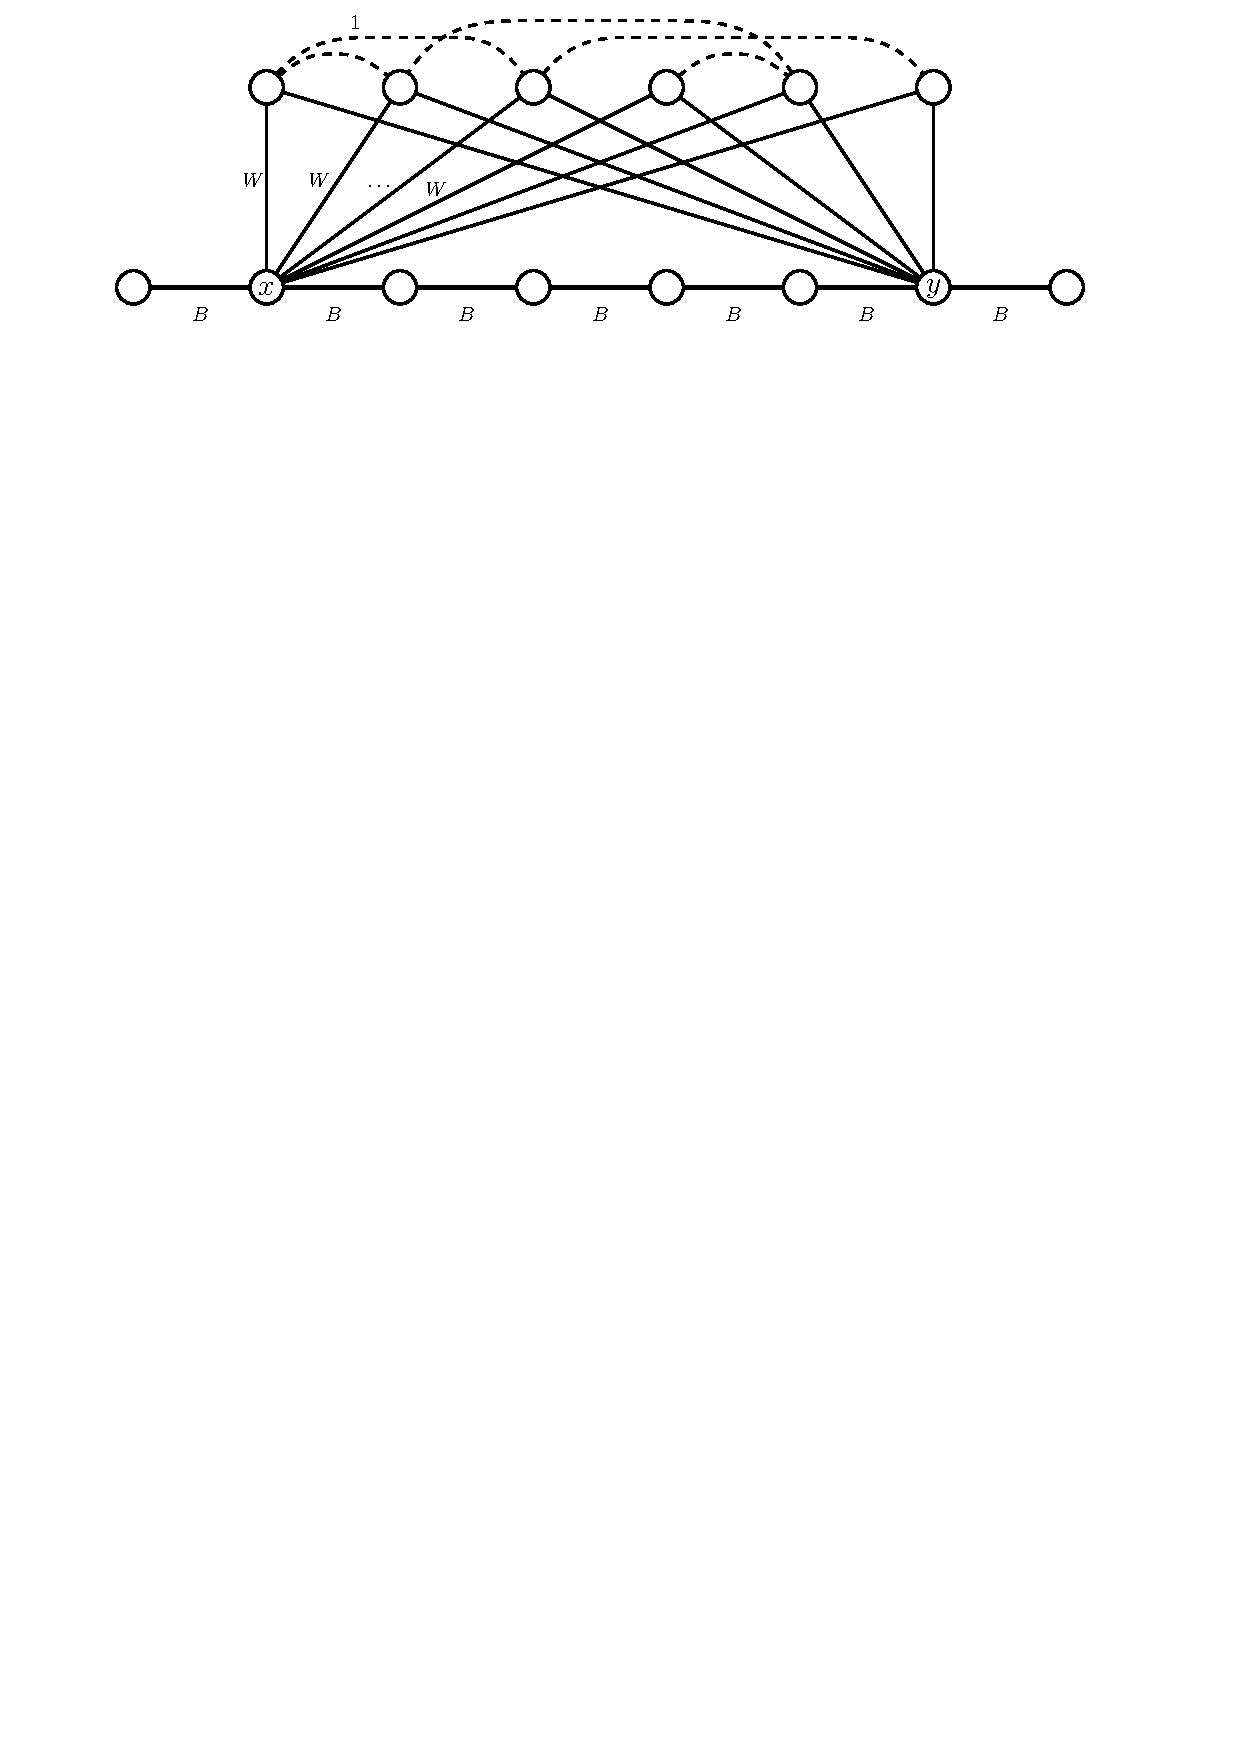
\includegraphics[width=0.3\textwidth]{figs/substitute}
	\caption{Cluster signatures in warm-up k=3 proof}
\end{figure}

\maciek{Rewrite: cluster types should be cluster signatures}
In our analysis, we distinguish among three types of clusters: $C_1, C_2, C_3$. In a cluster of type $C_i$, the size of the largest component contained in this cluster is $i$.
Before bounding the competitive ratio of \TAlg, we introduce the lemma that estimates the cost of a single repartition of \TAlg.

\begin{lemma}
	\label{lem:1req}
	During a single repartition, \TAlg exchanges at most $2$ pairs of nodes.
\end{lemma}

\begin{proof}
	Observe that when the repartition is triggered by \TAlg, the resulting partitioning is component respecting.
	Otherwise, if it does not exist, \TAlg simply ends the phase and performs no repartition.
	
	%We distinguish between three types of clusters: $C_1, C_2, C_3$,
	%which we define as follows.
	%A cluster of type $C_1$ the cluster contains $3$ singleton components (this is also the initial configuration of any cluster).
	%A cluster of type $C_2$  contains one component of size $2$ and one component of size $1$.
	%Finally, a cluster of type $C_3$  contains one component of size $3$.
	
	Consider a request between $u$ and $v$ that triggered the repartition and let $U$ and $V$ be their respective clusters.
	Note that $U\neq V$,
	as otherwise, the request would not trigger a~repartitioning.
	We consider cases based on the types of clusters $U$ and $V$.
	Note that this is impossible that either $U$ or $V$ is of type $C_3$, as otherwise, we merge components of size $3$, and no component respecting partitioning exists, a contradiction.
	If either $U$ or $V$ is of type $C_1$, then this cluster can fit the merged component, and the reconfiguration is local within $U$ and $V$.
	For two clusters, any configuration can be reached within two swaps, due to the fact that clusters are indistinguishable.
	
	Finally, we consider the case where both $U$ and $V$ are of type $C_2$. Note that $(u,v)$ cannot both belong to a component of size $2$, as this would mean that \TAlg has the component of size $4$, a contradiction with the case assumption that the component respecting partitioning exists. 
	Otherwise, if either $u$ or $v$ belongs to a component of size $2$, then it suffices to exchange components of size $1$ between $U$ and $V$.
	Finally, if $u$ and $v$ belong to components of size $1$, then we must place them in a cluster different from $U$ and $V$.
	Note that in such case, a $C_1$-type cluster $W$ exists, as otherwise no component respecting partitioning exists. In this case \TAlg performs one swap, i.e., it exchanges the nodes $u$ and $v$ with any two nodes of $W$.
\end{proof}

Corollary: DET2 is $O(\ell)$-competitive for $k=3$.

\subsection{Characterization of the migration graph}

Consider a component merge action performed by \TAlg that triggers a reconfiguration from a configuration $C_I$ to a configuration $C_F$.
To execute the reconfiguration, the nodes of two non-collocated components migrate to a common cluster.
Each cluster contains exactly $k$ nodes, thus other nodes migrate to take the place of nodes of merged components.
Their place must be occupied, too, and this way a single merge action may trigger migrations in clusters not directly involved in a merge action (for an example, see Section~\ref{ssec:example}). 
Recall that both $C_I$ and $C_F$ are component-respecting configurations, hence a migration of a single node entails migrations of all nodes of its cluster.

In Section~\ref{ssec:cascade}, we upper bound the cost incurred by a reconfiguration that follows a single component merge.
To this end, we introduce a \emph{migration graph} that models the reconfiguration.
In the following, we characterize the structure of the migration graph.

\noindent
\textbf{Vertices of the migration graph and the core vertices.}
The vertices of the migration graph are all $\ell$ clusters of the instance.
We distinguish the \emph{core vertices} that correspond to clusters directly involved in the merge operation: the clusters containing the to-be-merged components in $C_I$ and the cluster containing the merged component in $C_F$.
There are at most $3$ core vertices in each migration graph (at most two components participate in the merge, and these may migrate to a third cluster).

\noindent
\textbf{Edges and their labels.}
The edges of the migration graph denote the migration of nodes from $C_I$ to $C_F$.
Each edge is labeled with a number $m$ that denotes the number of migrated nodes between clusters.
Each edge is directed from the cluster that contained the nodes to the cluster they migrated to.
Both edges might exists between a pair of nodes, as whole components of nodes migrate, and the back-and-forth exchange may be needed for the configuration $C_F$ to be component-respecting.

\noindent
\textbf{Vertex degree.}
At most $k$ nodes may migrate from a cluster and at most $k$ nodes may migrate into a cluster.
Thus, the sum of the labels for both ingoing and outgoing edges of each vertex is at most $k$.
This implies that the number of ingoing and outgoing edges is also bounded by $k$.

\noindent
\textbf{Flow preservation.}
In any feasible configuration, each cluster contains exactly $k$ nodes.
Thus, for any vertex, the sum of labels of ingoing edges must equal the sum of labels of outgoing edges.
\maciek{Can we say that this implies that the graph is a circulation?}

\noindent
\textbf{Migration graph and the cost of reconfiguration.}
The cost of cluster reconfiguration equals the number of exchanged nodes multiplied by $\alpha$.
From the standpoint of a migration graph, this corresponds to the sum of labels on edges of the graph.
A trivial upper bound on the cost is the size of the connected component in the migration graph multiplied by $2\alpha k$.

\medskip

Note that for a single component merge, multiple migration graphs may exist, and multiple of them might have the optimal cost.
In Section \ref{ssec:cascade}, we show that among all migration graphs for given component merge, there exists an optimal graph with the bounded cycle length.
Combined with other properties, this allows to bound the size of the migration graph, and consequently bound the cost of each repartition, that results in a bound of the competitive ratio for \TAlg.

\subsection{Costly cluster reconfiguration example}
\label{ssec:example}



\begin{figure}[H]
	\centering
	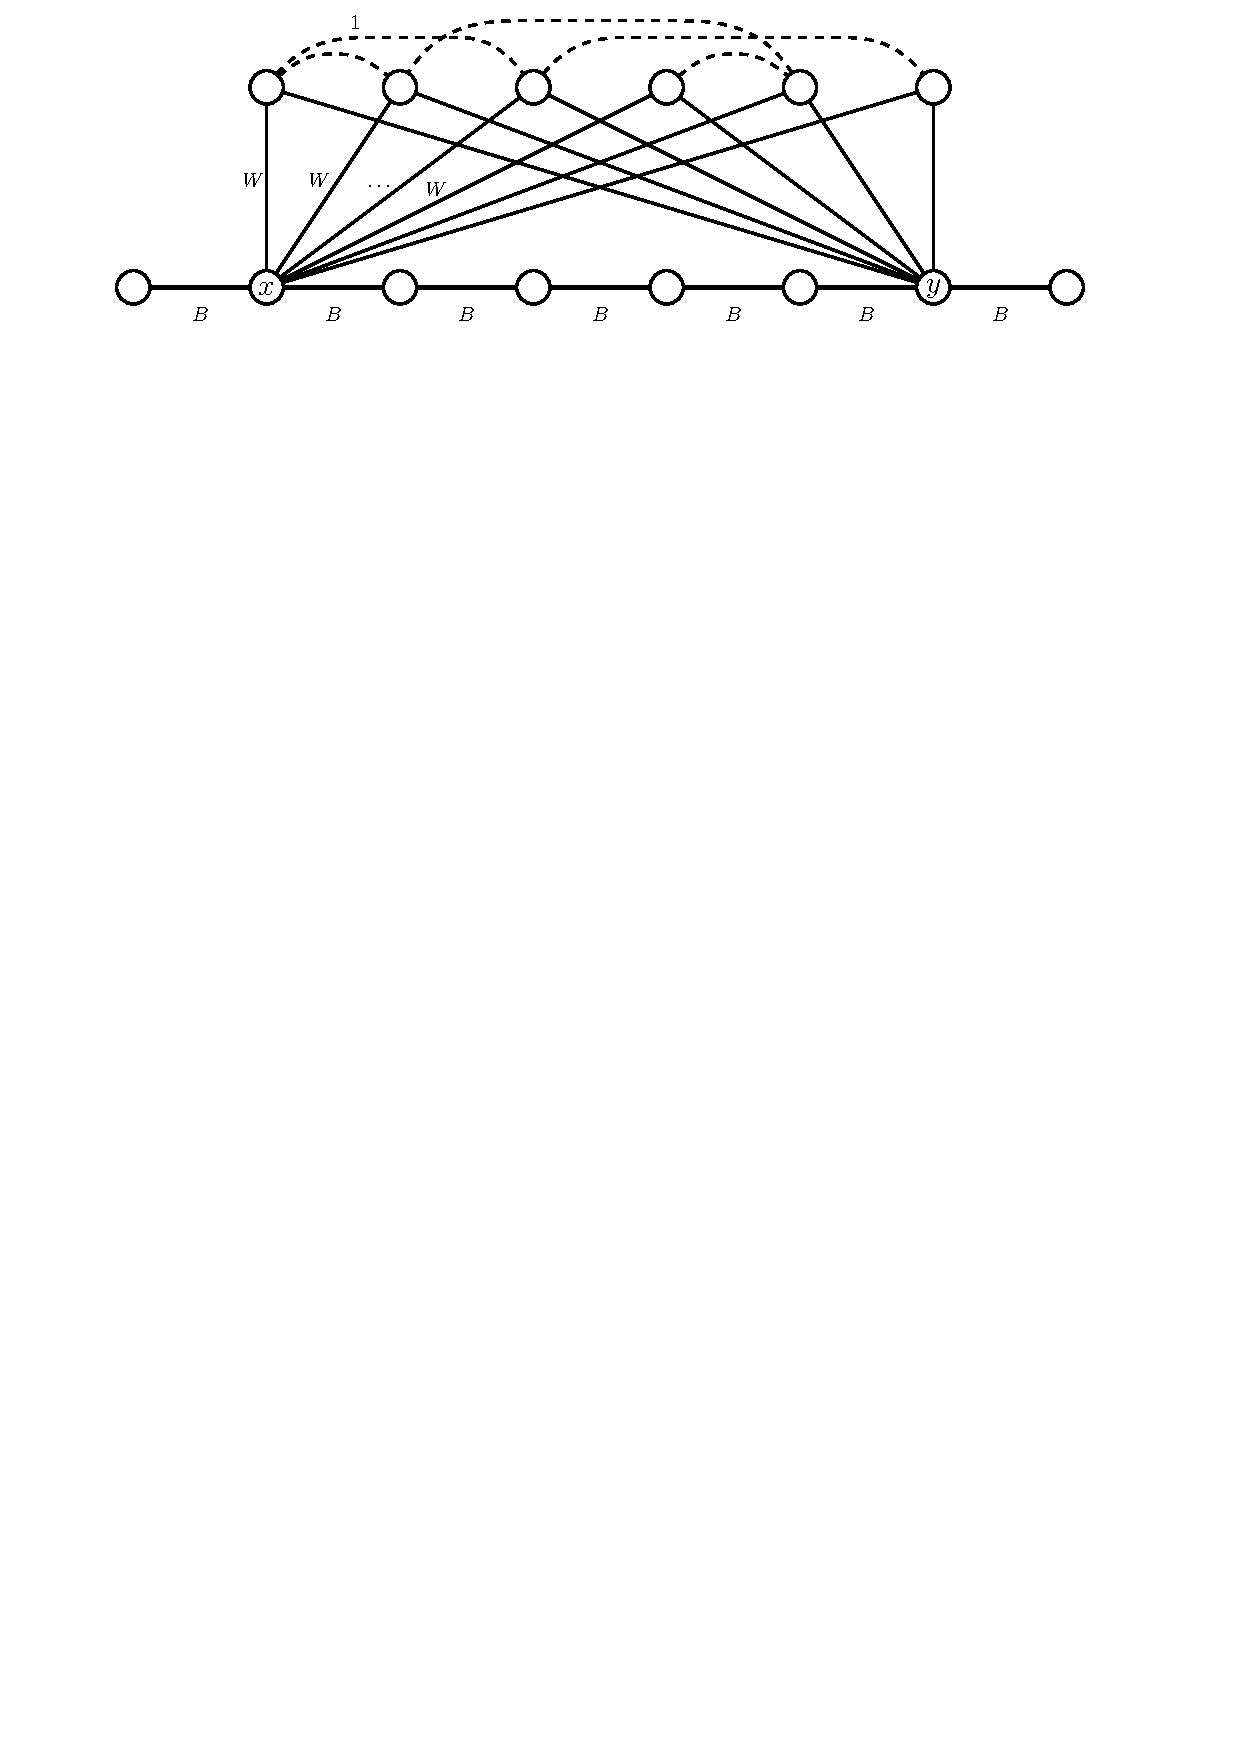
\includegraphics[width=0.3\textwidth]{figs/substitute}
	\caption{A costly cascade example. On the left: the configuration prior to the merge and the merge of two components (denoted solid). On the right: corresponding migration graph for the optimal (unique) reconfiguration.}
\end{figure}


In this section we present an example of a merge action that results in a $k/3$(?) length cycle in an optimal migration graph.

\subsection{Bounds on the size of a migration graph}
\label{ssec:cascade}

In \cite{repartition-disc}, authors trivially bounded the reconfiguration cost for each merge action by $k \cdot \ell$.
This roughly corresponds to migrating every node in every cluster.
Now, we bound the cost of a single repartition of \TAlg as a function of $k$.
Note that the bound of $k \cdot \ell$ is still valid, and the resulting bound is the minimum of these two.

We begin, by bounding the length of each cycle in one of optimal solutions.


\begin{figure}[H]
	\centering
	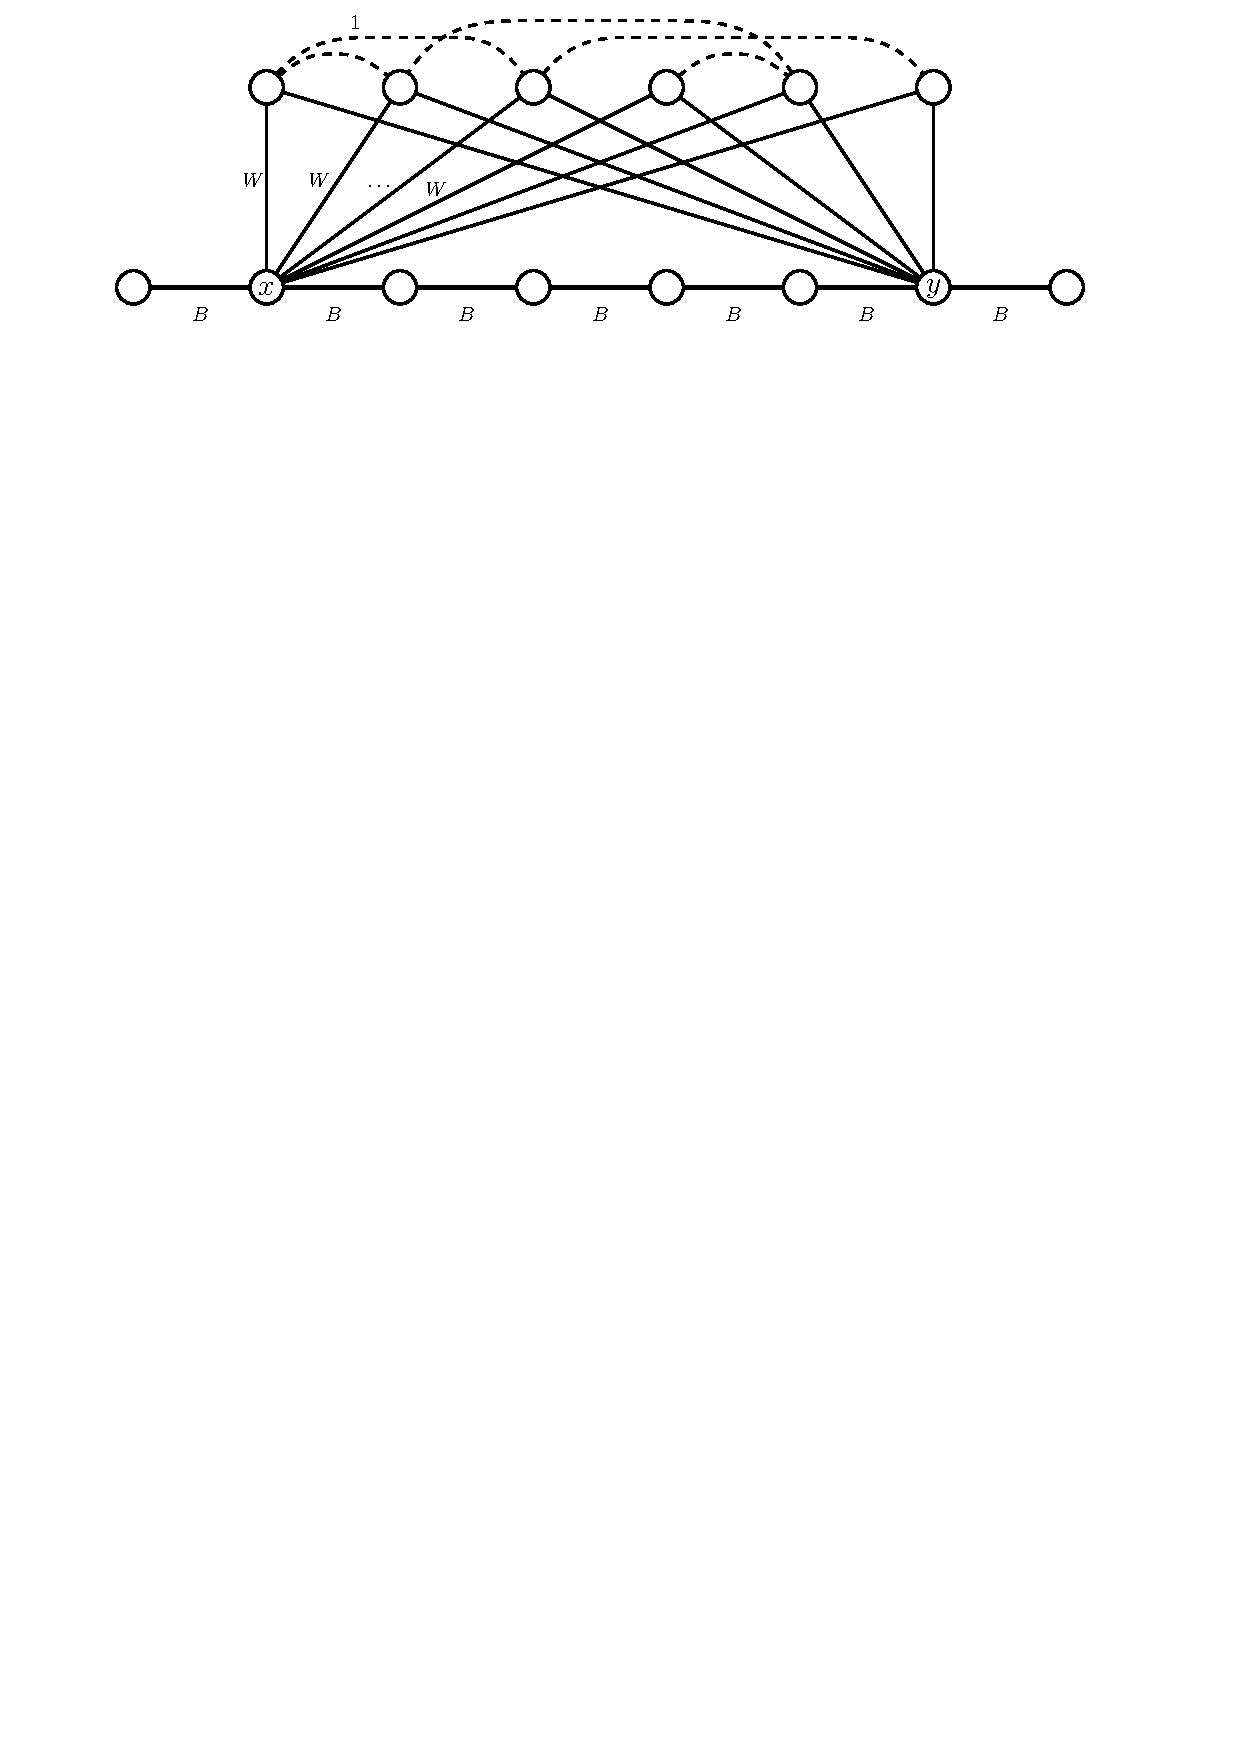
\includegraphics[width=0.3\textwidth]{figs/substitute}
	\caption{Illustration to bounding the cycle length.}
	\label{fig:cascade-illustration}
\end{figure}

\begin{theorem}
	\label{th:cascade-cycles}
	Consider a single merge action of \TAlg.
	There exists an optimal cost reconfiguration with the migration graph, where each cycle have length at most $k$.
\end{theorem}

\begin{proof}
	Assume the contrary, i.e., for each optimal cluster reconfiguration, its migration graph contains a cycle at least $k+1$.
	
	Fix a reconfiguration and its migration graph $G$ that has the shortest length $L$ of the longest cycle, and has the least number of cycles of length $L$.
	Let $p = \lbrace v_1, v_2, \ldots, v_L \rbrace$ be any cycle of length $L$.
	As edge labels are from $\{ 1, 2, \ldots, k \}$, there exists a pair of edges $e, f$ with equal labels.
	
	We show that in such case, we can modify the solution without affecting its cost and feasibility to decrease the number of cycles of length $L$ by $1$.
	This would contradict the assumption that we consider a solution with the minimal number of cycles of length $L$.
	
	We construct a new migration graph $G'$ of equal cost by swapping the (destination) endpoints of $e$ and $f$ (cf. Figure~\ref{fig:cascade-illustration})
	Formally, let $\lbrace a, b \rbrace = e$ and $\lbrace c, d \rbrace = f$.
	We remove $e$ and $f$ and add $e' = \lbrace a, d \rbrace$ and $f' = \lbrace c, d \rbrace$.
	This way we produced a feasible solution.
	
	It remains to show that while decreasing the number of cycles of length $L$, we did not created any new cycles of length at least $L$.
	Assume that adding $e'$ created a new cycle of length at least $L$.
	However, $a$ and $d$ were already connected in $G$ by a directed path of length at least $2$, and a cycle strictly longer than $L$ existed in $G$.
	
	Assume that adding $f'$ created a new cycle $s^*$ of length $L' \geq L$.
	Contrary to the previous case, the directed cycle from $e$ to $b$ might not exist in $G$.
	However, this would mean that $b$ and $e$ were connected by a path of length $L'-1$.
	This means that we might have followed this alternative path from $b$ to $e$ to obtain a cycle strictly longer than $L$ (cf. Figure~\ref{fig:cascade-illustration}).
	
\end{proof}


\begin{theorem}
	Consider a single repartition of DET2.
	The number of clusters it involves is bounded by $k^k$.
	\label{th:cascade}
\end{theorem}

\begin{proof}
	Each node has degree at most $k$.
	Every subset has flow conservation property, hence each cycle traverses one of the nodes of graph origin/core. (no subsets with just incoming edges to the origin part)
	Combine with Theorem \ref{th:cascade-cycles}.
	
\end{proof}


Corollary: Algorithm DET2 is $O(\ell \cdot k \cdot \min \{ \ell, k^k \})$-competitive.



\section{Improved algorithm for $k=2$}
\label{sec:k2}

\maciek{Intro: compare to previous 7-competitive algorithm. Note strict competitive ratio vs large additive term. Also, emphasize that in this section the algorithm is different than DET2}

Algorithm Alg:
maintain a counter $C_{\set{u,v}}$ for each pair of nodes $\set{u,v}$ and increment it on every remote request between $u$ and $v$.
Once $C_{\set{u,v}} = \lambda$,
reset the counter and collocate the pair arbitrarily in one of the two clusters where $u$ or $v$ resides.

\begin{theorem} \label{thm:k=2}
	The algorithm is (strictly) 6-competitive.
\end{theorem}


We charge both OPT and Alg whenever Alg collocates a pair (i.e., on a collocation event).
%More precisely,we charge them only the cost of the collocation, per such event.
%Hence,we charge the cost of  this collocation to OPT for the first time.
Alg collocates a pair always with a swap (i.e., two simultaneous migrations),
which  costs $2\alpha$.
%We charge OPT only for requests up to the one that triggers a collocation (i.e., not for later requests on the same pair).
OPT may save some costs by collocating multiple pairs at once (before they incur too much cost),
paying the price of only one migration per pair  (see Figure \ref{fig:TBD}).
%This observation suggests that we can't charge OPT more than $\alpha$ per collocation.
%E.g.,
%OPT can collocate two costly pairs with a single swap if
%it has both pairs on the cut of  the same two clusters.
%Later, Alg collocates those pairs with two swaps.
Hence,
whenever OPT collocates a pair,
we charge it only the cost of moving a single node to the cluster of the other,
i.e., $\alpha$ (in contrast to $2\alpha$ on Alg).


\begin{proof}[Proof of Theorem \ref{thm:k=2}]
	Assume on request $\sigma_{t}=\set{u,v}$, 
	i.e., at (time) $t$,
	Alg collocates the pair $\set{u,v}$.
	This means,
	the value of $C_{\set{u,v}}$ at $t$,
	denoted by $C^t_{\set{u,v}}$, 
	reaches $\lambda$ immediately before Alg resets the counter.
	I.e.,
	$ C^t_{\set{u,v}} = \lambda$.
	%	In case the first collocation of $\set{u,v}$ occurs at $t$,
	%	if the pair is collocated in the initial configuration then
	%	we set $t''=0$,
	%	else,
	%	we set $ t'' = -\infty, t'=0$.
	We denote the set of all requests to a pair $\set{x,y}$ that arrive
	during $(t_1,t_2]$ by $\sigma_{\set{x,y}}(t_1,t_2]$.
	
	If $t$ is the first time that Alg collocates $\{u,v\}$ then we  charge
	OPT $\lambda$ for serving requests in $\sigma_{\set{u,v}}[0,t]$ (remotely),
	or $\alpha$ for collocating the pair and serving them with no additional cost.
	Therefore in this case ,
	OPT pays $\min{\{ \lambda,\alpha \}}$.
	
	Else, we consider that Alg collocated $\{u,v\}$ in the past.
	Let $t'$, $t' < t$ be the  time when Alg separates $\set{u,v}$
	in order to collocate some (intersecting) pair
	$\{x,y\} \neq \{u,v\}, \{x,y\} \cap \{u,v\} \neq \emptyset$, 
	e.g.,
	$\{x,y\}=\{u,v'\}$.
	%	I.e., $ C^{t'}_{\set{u,v'}} = \lambda$.
	Similarly,
	if $t'$ is not the first time that Alg  collocates $\{u,v'\}$ 
	then let $t''<t'$ be the last time before $t'$ when Alg separates $\set{u,v'}$.
	Else,
	$\{u,v'\}$ is not collocated in the initial configuration and we let $t''=0$.
	By these definitions,
	we have
	$| \sigma_{\set{u,v'}}(t'',t'] | = | \sigma_{\set{u,v}}(t',t] |  =  \lambda$.
	The overall cost of requests in $\sigma_{\set{u,v}}(t',t]$,
	and the moving cost,
	incurred by Alg is
	$\lambda + 2\alpha$.
	Observe that for requests in $r_t := \sigma_{\{u,v'\}}(t'',t'] \cup \sigma_{\{u,v\}}(t',t]$,
	OPT must pay a total cost of serving and (or) migration at least
	$\min{ \{ 2\lambda, \lambda+\alpha, 2\alpha \} }$
	within $(0,m]$,
	regardless of its choices.
	%% 
	However,
	we cannot charge this cost to OPT repeatedly,
	i.e.,
	when Alg collocates the two pairs a second time.
	In particular,
	we charge OPT a cost incurred by requests in
	$\sigma_{\{u,v'\}}(t'',t']$ and $\sigma_{\{u,v\}}(t',t]$,
	if and only if  OPT incurs the cost within  intervals $(t'', t']$ and $(t', t]$,
	respectively.	
	Latter,
	this ensures us that we do not charge OPT for a cost more than twice.
	%%
	Based on this observation,
	we distinguish three cases of OPT's choices
	while it serves requests in	$r_t $.
	We denote its cost by
	$\mathit{Cost}_{\mathit{OPT}} (r_t) := \mathit{Cost}_{\mathit{OPT}} (\sigma_{\{u,v'\}}(t'',t']) 
	+ \mathit{Cost}_{\mathit{OPT}} (\sigma_{\{u,v\}}(t',t]) $.
	\begin{enumerate}[label=\roman*.]
		\item
		OPT collocates $\{u,v'\}$ at  $t''$, $\{u,v\}$  at $t'$,
		and keeps them so during $(t'',t']$ and $(t',t]$, respectively.
		Therefore it serves all requests in $r_t$ with no additional cost and
		$\mathit{Cost}_{\mathit{OPT}} (r_t) = 2\alpha$.
		\item
		OPT has $\{u,v\}$ ($\{u,v'\}$) already collocated at $t'$ ($t''$) as well as during $(t',t]$ ($(t'',t]$),
		and has $\{u,v'\}$ ($\{u,v\}$) separated during $(t'',t']$ ($(t',t]$).
		Hence,
		it pays only $\lambda$ for serving all requests in $r_t$ and
		$\mathit{Cost}_{\mathit{OPT}} (r_t) = \lambda$
		\item
		OPT has $\{u,v'\}$ ($\{u,v\}$) already  collocated at $t''$ ($t'$)  and also during $(t'',t']$ ($(t', t])$,
		and it collocates $\{u,v\}$ ($\{u,v'\}$) at $t'+1$ ($t''+1$) paying $\alpha$.
		%		Therefore it pays only $\alpha$ during $[t'',t]$,
		%		for collocating $\{u,v'\}$
		%	    and for the one request to $\{u,v\}$ at $t'$.
		%		I.e., it pays zero for every other  request in $r_t$.
		Then,
		$\mathit{Cost}_{\mathit{OPT}} (r_t) = \alpha$.
	\end{enumerate}
	In every of these cases,
	we have
	$\mathit{Cost}_{\mathit{OPT}} (r_t) \geq  \min{ \{ \lambda, \alpha \}}$.
	OPT may deviate from these cases,
	e.g.~by collocating a pair after partially paying for requests to this pair.
	However,
	no deviation can decrease the cost to OPT.
	\mahmoud{It would be better to describe and bound the "deviation" formally.}
	Therefore in any case,
	$\mathit{Cost}_{\mathit{OPT}} (r_t) \geq  \min{ \{ \lambda, \alpha \}}$.
	
	It remains to charge both Alg and OPT for requests that do not lead to collocations until the  end of the sequence at $t=m$.
	Assume $\{u,v\}$ is not collocated at $t=m$
	and $0 < C^{m}_{ \{u,v\} } < \lambda $,
	which means Alg pays $C^{m}_{ \{u,v\} }$
	for requests to $\{u,v\}$ so far unaccounted.
	If $\{u,v\}$ is not collocated in the initial configuration
	and Alg never collocates it through the sequence,
	then $ C^{m}_{ \{u,v\} } =| \sigma_{\{u,v\}}[1,m] |$.
	We charge OPT the cost
	$\mathit{Cost}_{\mathit{OPT}} (\sigma_{\{u,v\}}[1,t]) 
	\geq \min{ \{ \alpha, C^{m}_{ \{u,v\} } \} }$,
	for collocating this pair or (and) paying (partially) for requests in $\sigma_{\{u,v\}}[1,t]$.
	Else,
	either $\{u,v\}$ is collocated in the initial configuration
	or Alg collocates it at some point.
	Then there exists an intersecting pair $\set{u,v'}$
	that is collocated by Alg at $t' < m$ (separating $\{u,v\}$).
	We define times $t'' < t' < m$ similarly to the case where Alg collocates $\{u,v\}$.
	Let $r_{\{u,v\}} := \sigma_{\{u,v'\}} (t'',t'] \cup \sigma_{\{u,v\}} (t',m]$.
	Then,
	we apply cases (i) to (iii) in an analogous way,
	replacing $\lambda$ with $C^{m}_{ \{u,v\}}$ in the analysis.
	Thus, 
	we obtain
	$\mathit{Cost}_{\mathit{OPT}} (r_{\{u,v\}}) 
	\geq  \min{ \{ C^{m}_{ \{u,v\}}, \alpha \}}$.
	
	Next, we sum up all costs charged to OPT.
	Observe that by definition,
	$r_{t'} \cap r_t = \sigma_{\{u,v'\}}[t'',t']$.
	This means,
	the cost of r.h.s.~to OPT is counted at most twice in the expression
	$\mathit{Cost}_{\mathit{OPT}} (r_{t'}) + \mathit{Cost}_{\mathit{OPT}} (r_t)$.
	Hence,
	for all collocations performed by Alg,
	and for final costs at $t=m$,
	OPT pays at least 
	$(
	\sum_{ 0 < t \leq |\sigma|} \mathit{Cost}_{\mathit{OPT}} (r_t) +
	\sum_{\{u,v\}} \mathit{Cost}_{\mathit{OPT}} (r_{\{u,v\}})
	) / 2$.
	Let
	$T := \{ 0 < t \leq m ~\vert~ \exists \{u,v\}: C^{t}_{\{u,v\}} = \lambda \}$.
	By setting $\lambda= \alpha$,
	we obtain
	\begin{align*}
		\mathit{Cost}_{\mathit{ALG}} (\sigma)	/
		\mathit{Cost}_{\mathit{OPT}} (\sigma)
		&=
		\Big(
		\sum_{ t \in T}(\lambda + 2\alpha) +
		\sum_{\{u,v\}} C^{m}_{\{u,v\}}
		\Big)	 \big /
		\frac{1}{2}
		\Big(
		\sum_{ t \in T} \mathit{Cost}_{\mathit{OPT}} (r_t) 
		+ \sum_{\{u,v\}}\mathit{Cost}_{\mathit{OPT}} (r_{\{u,v\}})
		\Big)	\\
		&\leq
		\Big(
		\sum_{ t \in T}(\lambda + 2\alpha) +
		\sum_{\{u,v\}} C^{m}_{\{u,v\}}
		\Big)	 \big /
		\frac{1}{2}
		\Big(
		\sum_{ t \in T} \min{ \{ \lambda, \alpha \}}  +
		\sum_{\{u,v\}} \min{ \{C^{m}_{\{u,v\}} , \alpha \} } 
		\Big)	\\
		&=
		2\Big(
		\sum_{ t \in T} 3\alpha +
		\sum_{\{u,v\}} C^{m}_{\{u,v\}}
		\Big)	 \big /
		\Big(
		\sum_{ t \in T} \alpha  
		+ \sum_{\{u,v\}} C^{m}_{\{u,v\}}  
		\Big)	< 6
	\end{align*}.
	%	The claim follows from here.
\end{proof}

Major:

\maciek{I feel slightly uneasy here: "In particular,
we charge OPT a cost incurred by requests in
$\sigma_{\{u,v'\}}(t'',t']$ and $\sigma_{\{u,v\}}(t',t]$,
if and only if  OPT incurs the cost within  intervals $(t'', t']$ and $(t', t]$,
respectively.	"}

\maciek{"Observe that for requests in $r_t$". First the separate sentence with the definition of $r_t$ (it is challenging enough to just understand it. Then reason why it pays the minimum of three values (I don't see it, and later you show that cost(rt) is at least minimum of other two values). Is it a consequence of three cases?}

\maciek{"We charge OPT the cost
$\mathit{Cost}_{\mathit{OPT}} (\sigma_{\{u,v\}}[1,t]) 
\geq \min{ \{ \alpha, C^{m}_{ \{u,v\} } \} }$,
for collocating this pair or (and) paying (partially) for requests in $\sigma_{\{u,v\}}[1,t]$." No issues with charge sharing from "regular collocation" case? Maybe I just don't understand "partially" here. Not necessarily rewrite! Just maybe check if it's true.}

Minor:

\maciek{Remove all "charge both". Just sum up costs. I would say not use "charge" at all, but it's up to you.}


\maciek{Structure in paragraphs. 3 parts: first collocation, regular collocation and unfinished. Do this for ALG and then for OPT, and do not mix (unless I don't see some dependencies). Start each paragraph by the sentence that says what the paragraph is about (first/opt, regular/alg etc.). Assume that the reader reads only the first sentence of each paragraph (if it's short), and the proof structure must be clear from this. Some other important things go to their own paragraph too, and the first sentence must describe what we do there.}

\maciek{$r_t$ is the central concept in this proof. Possibly even start with the paragraph: charging OPT, regular collocation. Make this definition in its separate line to further emphasize? It would suffice for a profesional to see the definiton of $t''/t'$ and this line to convince himself that the proof is correct.}

\maciek{I think that "deviate" is OK to use like this.}

Notation:

\maciek{End of the time proposition: $t_e / t^* / T$ instead of $m$? Or capital $T$ (but I am aware of the conflict)}

\maciek{Instead of $cost_{opt}$ just use opt / alg?}

\maciek{Consider naming the adjacent edges $e$ and $f$.}

\begin{comment}
	We charge both OPT and Alg whenever Alg collocates a pair (i.e., on a collocation event).
	%More precisely,we charge them only the cost of the collocation, per such event.
	%Hence,we charge the cost of  this collocation to OPT for the first time.
	Alg collocates a pair always with a swap (i.e., two simultaneous migrations),
	which  costs $2\alpha$.
	%We charge OPT only for requests up to the one that triggers a collocation (i.e., not for later requests on the same pair).
	OPT may save some costs by collocating multiple pairs at once (before they incur too much cost),
	paying the price of only one migration per pair.
	This observation suggests that we can't charge OPT more than $\alpha$ per collocation,
	even when OPT actually pays more than that.
	E.g.,
	OPT can collocate two costly pairs with a single swap if
	it has both pairs on the cut of  the same two clusters.
	Later, Alg collocates those pairs with two swaps (see Figure \ref{fig:TBD}).
	Hence,
	whenever OPT collocates a pair,
	we charge OPT only the cost of moving a single node to the cluster of the other,
	i.e., $\alpha$ (in contrast to $2\alpha$ for Alg).
	
	\begin{proof}[Proof of Theorem \ref{thm:k=2}]
		\mahmoud{not correct}
		%	Let $C^{t}_{\set{u,v}}$ denote the  value of $C_{\set{u,v}}$
		%	immediately after arrival of the $t$th request,
		%	$\sigma_t$.
		Assume on request $\sigma_{t}=\set{u,v}$, 
		i.e., at (time) $t \geq 1$,
		Alg collocates the pair $\set{u,v}$.
		This means,
		the value of $C_{\set{u,v}}$ at $t$,
		immediately before Alg resets the counter is $\lambda$.
		That is, $ C^t_{\set{u,v}} = \lambda$.
		Let $\sigma_{t''}, t''<t$ be the last request (before $\sigma_{t}$)
		upon which Alg collocates $\set{u,v}$.
		Let $t'$, $t'' < t' < t$ be the  time when Alg separates $\set{u,v}$
		in order to collocate some other pair that shares a node with $\set{u,v}$,
		e.g.~$\set{u,v'}, v' \neq v$.
		In case the first collocation of $\set{u,v}$ occurs at $t$,
		if the pair is collocated in the initial configuration then
		we set $t''=0$,
		else,
		we set $ t'' = -\infty, t'=0$.
		We denote the set of all requests to $\set{u,v}$
		during $[t_1,t_2]$ by $\sigma_{\set{u,v}}[t_1,t_2]$.
		Thus,
		$| \sigma_{\set{u,v}}[t',t] | = \lambda$.
		The overall cost of requests that increase the counters of intersecting pairs,
		%	i.e.~requests in $\sigma_{\set{u,v}}[t'',t]$,
		and the moving cost,
		incurred by Alg is
		$\lambda + 2\alpha$.
		%That is, the cost of all requests in $\sigma_{\set{u,v}}[t',t]$.
		
		We distinguish three cases for the cost incurred by OPT with respect to the collocation of $\set{u,v}$ at $t$.
		
		\begin{enumerate}
			\item Case i)
			OPT has $\set{u,v}$ separated (in OPT's configuration) during $[t',t]$
			and therefore it pays $\lambda$.
			We charge OPT $\lambda/2$, i.e.,
			$\mathit{Cost}^{t}_{\{u,v\}} (\mathit{OPT})= \lambda / 2$.
			
			
			\item Case ii)  
			OPT collocates $\set{u,v}$ some time during $[t'',t]$ and pays $\alpha$.
			We charge it $\alpha/2$, i.e.,
			$\mathit{Cost}^{t}_{\{u,v\}} (\mathit{OPT}) = \alpha / 2$.
			
			
			\item Case iii)
			$t'' \geq 0$ and OPT has $\set{u,v}$ already collocated before $t''$.
			%	 and keeps them collocated during $[t'',t]$.
			In this case,
			OPT possibly pays zero for requests in $\sigma_{\set{u,v}}[t'',t]$.
			However,
			by assumption,
			Alg collocates $\{u,v'\}$ at $t'$ and
			OPT doesn't have $\{u,v'\}$ collocated through the entire
			$[\tau^{t''}_{\{u,v'\}}, t']$.
			This implies that only cases (i) or (ii) applies to $\{u,v'\}$ at $t'$.
			That is,
			OPT pays $\min \{ \lambda, \alpha \}$,
			and it is charged $\min \{ \lambda/2, \alpha/2 \}$
			w.r.t.~the collocation of $\{u, v'\}$ at $t'$.
			Hence,
			we can charge it  $\min \{ \lambda/2, \alpha/2 \}$ in addition to the  cost already charged.
			%	i.e.~the remaining (unaccounted) cost of requests in $\sigma_{\set{u,v'}}[t'',t']$.
			%	Intuitively, at $t$,  we charge $\alpha$ to OPT for separating $\set{u,v}$ (at $t'$) by Alg.
		\end{enumerate}
		
		It can be easily verified that any deviation from these cases only increases the cost to OPT.
		Thus,
		OPT pays at least $\alpha$ for each collocation performed by Alg.
		%	which gives the competitive ratio 
		%	$(\lambda + 2\alpha)/ \alpha = 4$.
		
		It remains to charge both Alg and OPT for requests that do not lead to collocations when the sequence ends.
		Consider  pairs $\set{u,v}$ and $\set{u,v'}$ and
		times $t'' < t' < t = t_m$ as defined previously.
		Assume $\sigma_{\set{u,v}}[t'', t_m] \leq \lambda - 1$.
		This means Alg has the pair separated at $t_m$
		and paid the (communication) cost $r_{\set{u,v}} := | \sigma_{\set{u,v}}[t'', t_m]|$.
		If OPT has the pair separated during $[t'',t_m]$ then it pays $r_{\set{u,v}}$.
		If OPT collocates the pair some time during $[t'', t]$ then analogous to Case (ii),
		we charge it $\alpha$.
		Otherwise,
		if OPT collocates the pair before $t''$,
		then we charge it $\alpha$ analogously to Case (iii).
		Hence, 
		$Cost(OPT)_{\set{u,v}} / Cost(Alg)_{\set{u,v}} =
		\max \set{ r_{\set{u,v}}/ \alpha \leq (\lambda-1) / \alpha , (\lambda + 2\alpha)/ \alpha} = 4$.
		%	The claim follows from here.
	\end{proof}
\end{comment}

\section{Note on distributed algorithms}


\subsection{Distributed implementation of $k=3$ algorithm}

For a repartition, it is sufficient to find the cluster with the signature $1,1,1$. 
We call any such cluster \emph{X (todo name)}.
Idea of distributed implementation of this procedure:
\begin{enumerate}
	\item Assign ids to clusters and order them
	\item Recursively partition clusters into two groups
	\item Each group maintains the pointer to a subgroup that contains at least one X cluster; a pointer may be null (then no X there)
	\item This way, finding a cluster X requires $\log_2(\ell)$ communication
	\item After removing an X cluster, we need to fix the pointers. This is done by following the path from the removed X cluster to the root. We simply ask the sibling if it contains X.
	\item Possible improvement: we can have a fixed number of rounds for finding the X cluster by maintaining a direct pointer to an X cluster (not only to subgroup). However, the fix still requires the log number of rounds. But we improved the responsiveness.
\end{enumerate}

\subsection{Distributed implementation of $k=2$ algorithm}

Trivial? Counters are local. We migrate between the clusters that have just communicated.

\subsection{Distributed implementation of PPL}

\maciek{How to distribute PPL better?}

Our algorithms can be distributed
similarly to the approach in~\cite{sigmetrics19_partitioning}.

\bibliographystyle{ACM-Reference-Format}
\bibliography{references}  

\pagebreak
\appendix


\section{Omitted results}

\begin{enumerate}
	\item The lower bound of $\Omega(\ell)$ for the scenario with at most $(1/3-1/k)$-augmentation
	
	\item Costly cascade example (it is easy to present $k^2$ and $k\cdot \sqrt{k}$ (with different approach), and then we can combine these to obtain $k^3$)
	
	\item $k$-competitive algorithm for the ring communication pattern
	
	\item lower and upper bound $k+1$ for two clusters, perfect partition and the optimal configuration reachable within one swap
	\item 
	The bound $(k \cdot \ell - k - \ell) / 2$ can be easily improved to $(k \cdot \ell - k - 1) / 2$ by playing a simple caching game in the first cluster, instead of just giving away the $k-1$ "blocker" (the caching game would build it gradually)
	
\end{enumerate}


\end{document}
